% !TEX root = ../main.tex
\chapter{Theory of heavy ion collisions}
  %
  % ========
  \section{The Standard Model}
  % ========
    In the 1970s, a new theory of fundamental particles and their interaction emerged.
    A new concept, which concerns the electromagnetic, weak and strong nuclear interactions between know particles.
    This theory is called \textit{The Standard Model}.
    There are seventeen named particles in the standard model, organized into the chart shown below (Fig. \ref{fig:standard_model}).
    Fundamental particles are divided into two families: \textit{fermions} and \textit{bosons}.
     \begin{figure}[h]
       \centering
       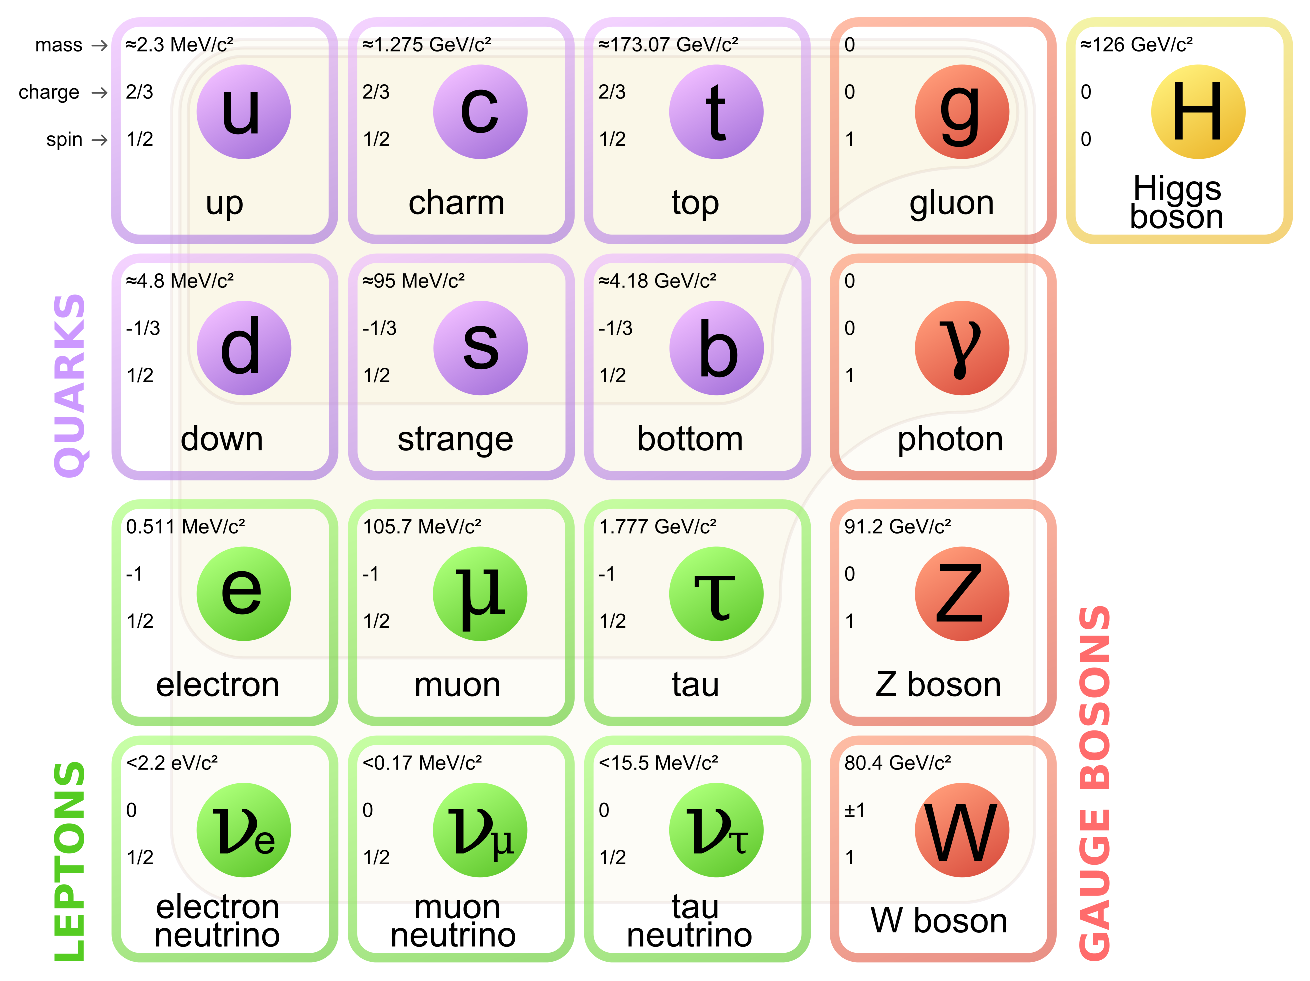
\includegraphics[width=0.9\textwidth]{standard_model}
       \caption{The Standard Model of elementary particles~\cite{sm_svg}.}
       \label{fig:standard_model}
     \end{figure}
     
    Fermions are the building blocks of matter.
    They are divided into two groups.
    Six of them, which must bind together are called \textit{quarks}.
    Quarks are known to bind into doublets (\textit{mesons}), triplets (\textit{baryons}) and recently confirmed four-quark states.\footnote{The LHCb experiment at CERN in Geneva confirmed recently existence of $Z$(4430) - a particle consisting of four quarks~\cite{fourquark}.}
    Two of baryons, with the longest lifetimes, are forming a nucleus: a proton and a neutron.
    A proton is build from two up quarks and one down, and neutron consists of two down quarks and one up.
    A proton is found to be a stable particle (at least it has a lifetime larger than $10^{35}$ years) and a free neutron has a mean lifetime about $8.8\times10^2$ s.
    Fermions, that can exist independently are called \textit{leptons}.
    Neutrinos are a subgroup of leptons, which are only influenced by weak interaction.
    Fermions can be divided into three generations (three columns in the Figure \ref{fig:standard_model}).
    Generation I particles can combine into hadrons with the longest life spans. 
    Generation II and III consists of unstable particles which form also unstable hadrons. 
    
    Bosons are force carriers.
    There are four fundamental forces: weak - responsible for radioactive decay, strong - coupling quarks into hadrons, electromagnetic - between charged particles and gravity - the weakest, which causes the attraction between particles with a mass.
    The Standard Model describes the first three.
    The weak force is mediated by $W^{\pm}$ and $Z^0$ bosons, electromagnetic force is carried by photons $\gamma$ and the carriers of a strong interaction are gluons \textit{g}.
    The fifth boson is a Higgs boson which is responsible for giving other particles mass. 
 
  %
  % ========
  \section{Quantum Chromodynamics}
  % ========
    %
    % ========
    \subsection{Quarks and gluons}
    % ========
      Quarks interact with each other through the strong interaction.
      The mediator of this force is a \textit{gluon} - a massless and chargeless particle.
      In the quantum chromodynamics (QCD) - theory describing strong interaction - there are six types of ``charges'' (like electrical charges in the electrodynamics) called \textit{colours}.
      The colors were introduced because some of the observed particles, like $\Delta^{-}$, $\Delta^{++}$ and $\Omega^{-}$ appeared to consist of three quarks with the same flavour (\textit{ddd}, \textit{uuu} and \textit{sss} respectively), which was in conflict with the Pauli principle.
      One quark can carry one of the three colors (usually called \textit{red}, \textit{green} and \textit{blue}) and antiquark one of the three anti-colors respectively.
      Only color-neutral (or white) particles could exist, mesons are assumed to be a color-anticolor pair, while baryons are \textit{red-green-blue} triplets.
      Gluons also are color-charged and there are 8 types of gluons.
      Therefore they can interact with themselves~\cite{perkins}.
    %
    % ========
    \subsection{Quantum Chromodynamics potential}
    % ========
      As a result of that gluons are massless, one can expect, that the static potential in the QCD will have the similar form like one in the electrodynamics e.g. $\sim 1/r$.
      In reality the QCD potential is assumed to have the form of~\cite{perkins}
      \begin{equation}
        V_s = - \frac{4}{3} \frac{\alpha_s}{r} + kr~,
        \label{eq:qcd_potential}
      \end{equation}
      where the $\alpha_s$ is a coupling constant of the strong force and the $kr$ part is related with the \textit{confinement}.
      In comparison to the electromagnetic force, a value of the strong coupling constant is $\alpha_s \approx 1$ and the electromagnetic one is $\alpha = 1/137$.

      The fact that quarks does not exist separately, but they are always bound, is called a confinement.
      As two quarks are pulled apart, the linear part $kr$ in the eq.~\ref{eq:qcd_potential} becomes dominant and the potential becomes proportional to the distance.
      This situation resembles stretching of a string.
      At some point, when the string is so large it is energetically favourable to create a quark-antiquark pair.
      At this moment such pair (or pairs) is formed, the string breaks and the confinement is preserved (Fig. \ref{fig:string_break}).
      \begin{figure}[h]
        \centering
        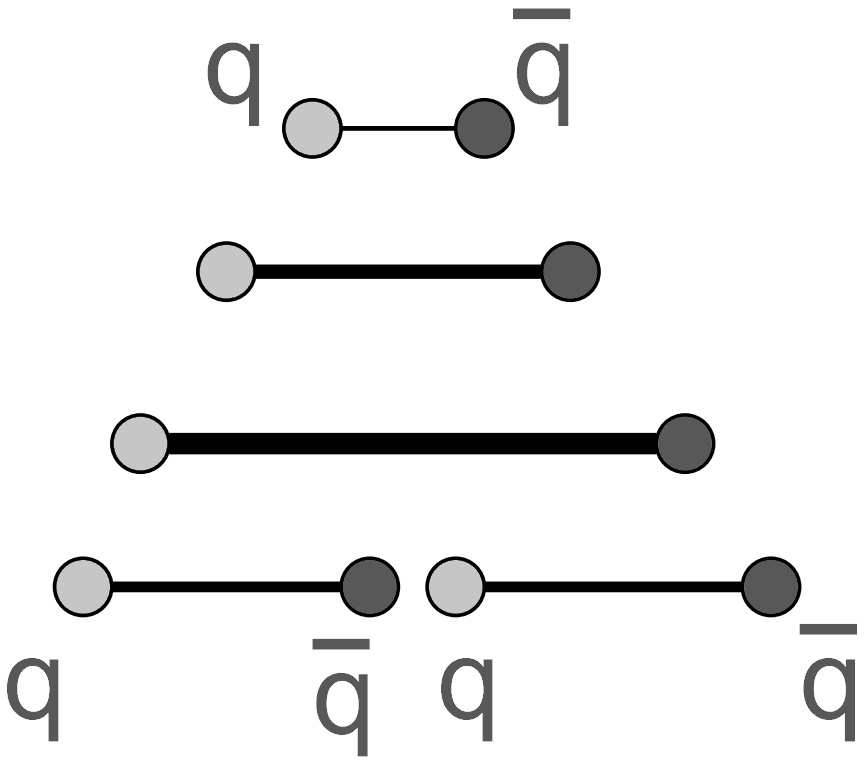
\includegraphics[width=0.25\textwidth]{string_break}
        \caption{A string break and a creation of a pair quark-anti-quark~\cite{dfck}.}
        \label{fig:string_break}
      \end{figure}
      
      On the other hand, for the small $r$, an interaction between the quarks and gluons is dominated by the Coulomb-like term $-\frac{4}{3} \frac{\alpha_s}{r}$.
      The coupling constant $\alpha_s$ depends on the four-momentum $Q^2$ transferred in the interation.
      This dependence is presented in Fig.~\ref{fig:strong_cc}.
      \begin{figure}[h]
        \centering
        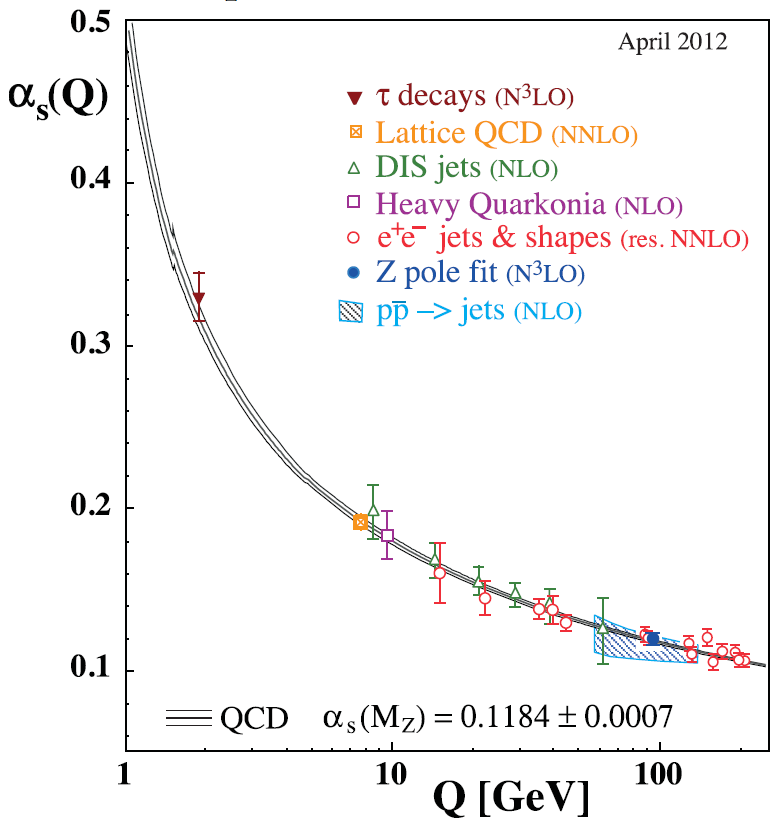
\includegraphics[width=0.5\textwidth]{strong_cc}
        \caption{Alpha.~\cite{pdg}.}
        \label{fig:strong_cc}
      \end{figure}
      The value $\alpha_s$ decreases with increasing momentum transfer and the interaction becomes weak for large $Q^2$ ($\alpha_s (Q) \to 0$).
      Because of weakening of coupling constant, quarks at large energies (or small distances) are starting to behave like free particles.
      This phenomenon is known as an \textit{asymptotic freedom}.      
      The QCD potential has also temperature dependence - the force strength ``melts'' with the temperature increase.
      Therefore the asymptotic freedom is expected to appear in either the case of high baryon densities (small distances between quarks) or very high temperatures.
      This temperature dependence is illustrated in the Fig.~\ref{fig:qcd_potential}.
      \begin{figure}[h]
        \centering
        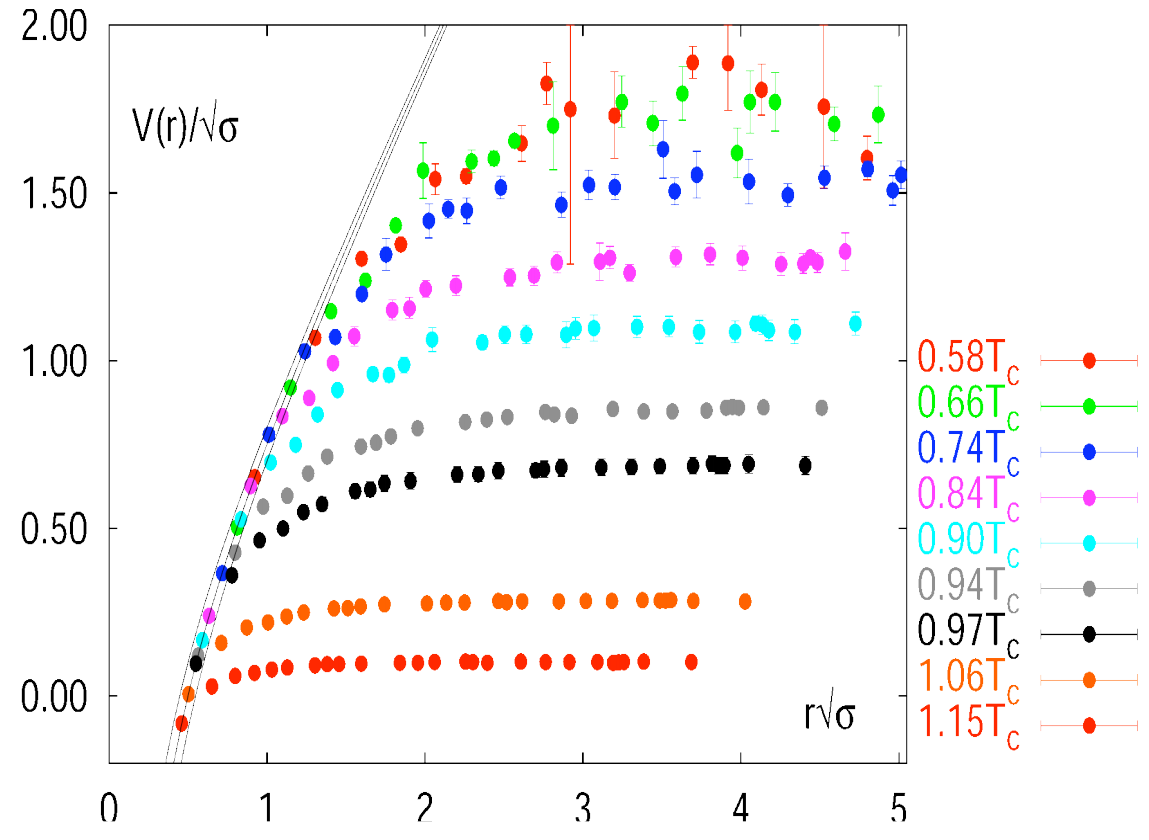
\includegraphics[width=0.62\textwidth]{qcd_potential_t}
        \caption{The QCD potential for a pair quark-antiquark as a function of distance for different temperatures.~\cite{dfck}.}
        \label{fig:qcd_potential}
      \end{figure}
      
      If the coupling constant $\alpha_s$ is small, one can use perturbative methods to calculate physical observables.
      Perturbative QCD (pQCD) successfully describes hard processes (with large $Q^2$), such as jet production in high energy proton-antiproton collisions.
      The applicability of pQCD is defined by the \textit{scale parameter} $\Lambda_{QCD} \approx$~200~MeV.
      If $Q \gg \Lambda_{QCD}$ then the process is in the perturbative domain and can be described by pQCD.
      A description of soft processes (when $Q <$~1~GeV) is a problem in QCD - perturbative theory breaks down at this scale.
      Therefore, to describe processes with low $Q^2$, one has to use alternative methods like Lattice QCD.
      Lattice QCD (LQCD) is non-perturbative implementation of field theory in which QCD quantities are calculated on a discrete space-time grid.
      LQCD allows to obtain properties of matter in equilibrium, but there are some limitations.
      Lattice QCD requires fine lattice spacing to obtain precise results - therefore large computational resources are necessary.
      With the constant growth of computing power this problem will become less important.
      The second problem is that lattice simulations are possible only for baryon density $\mu_B = $~0.
      At $\mu_B \neq 0$, Lattice QCD breaks down because of the sign problem~\cite{qcd_fodor}.
      
    %
    % ========
    \subsection{The quark-gluon plasma}
    % ========
      The new state of matter in which quarks are no longer confined is known as a \textit{quark-gluon plasma} (QGP).
      The predictions coming from the discrete space-time Lattice QCD calculations reveal a phase transition from the hadronic matter to the quark-gluon plasma at the high temperatures and baryon densities.
      \begin{figure}[h]
        \centering
        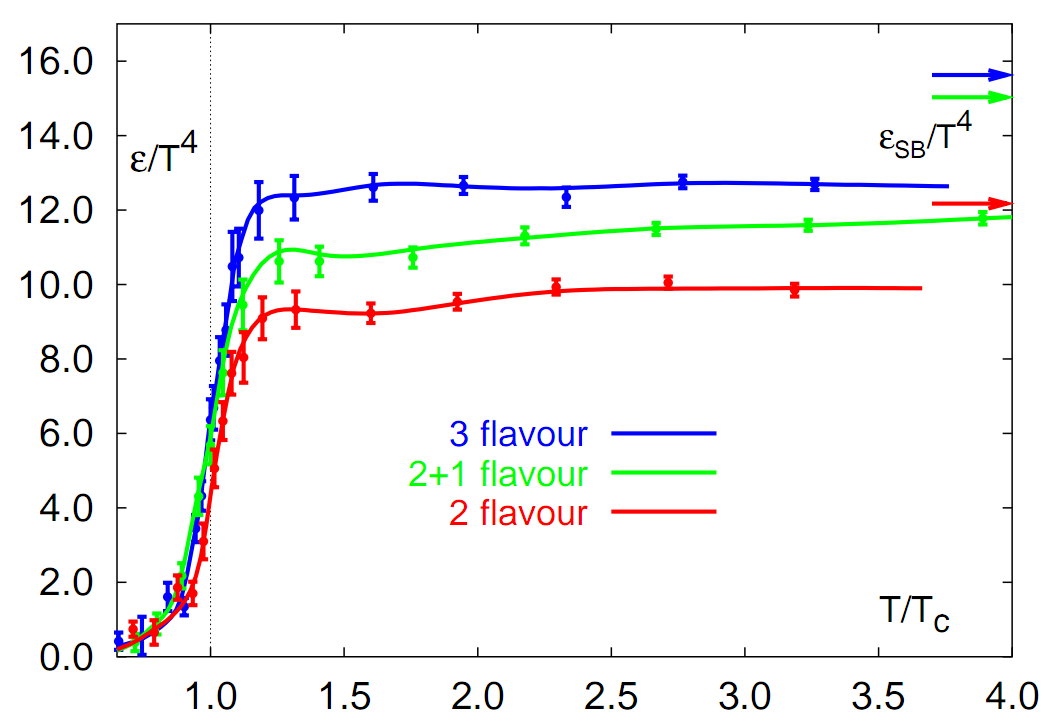
\includegraphics[width=0.6\textwidth]{lqcd}
        \caption{A number of degrees of freedom as a function of a temperature~\cite{karsch}.}
        \label{fig:lqcd}
      \end{figure}
      The results obtained from such calculations are show on Fig.~\ref{fig:lqcd}.
      The energy density $\epsilon$ which is divided by $T^4$ is a measure of number of degrees of freedom in the system.
      One can observe significant rise of this value, when the temperature increases past the critical value $T_C$.
      Such increase is signaling a phase transition - the formation of QGP~\cite{drkisiel}.
      The values of the energy densities plotted in Fig.~\ref{fig:lqcd} do not reach the Stefan-Boltzmann limit $\epsilon_{SB}$ (marked with arrows), which corresponds to the ideal gas.
      This can indicate some residual interactions in the system.
      According to the results from the RHIC\footnote{Relativistic Heavy Ion Collider at Brookhaven National Laboratory in Upton, New York}, the new phase of matter behaves more like an ideal fluid, than like a gas~\cite{bartke}.
      \begin{figure}[h]
        \centering
        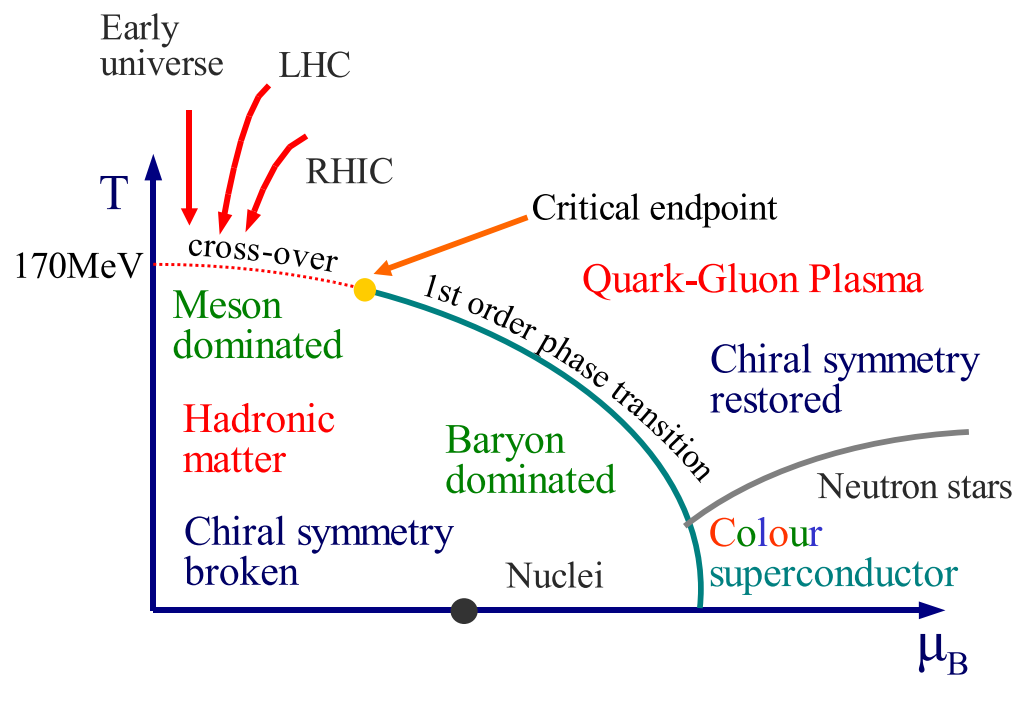
\includegraphics[width=0.7\textwidth]{phase_diagram}
        \caption{Phase diagram coming from the Lattice QCD calculations~\cite{drkisiel}.}
        \label{fig:phase_diagram}
      \end{figure}

      One of the key questions, to which current heavy ion physics tries to find an answer is the value of a critical temperature $T_C$ as a function of a baryon chemical potential $\mu_B$ (baryon density), where the phase transition occur.
      The results coming from the Lattice QCD are presented in the Fig.~\ref{fig:phase_diagram}.
      The phase of matter in which quarks and gluons are deconfined is expected to exist at large temperatures.
      In the region of small temperatures and high baryon densities, a different state is supposed to appear - a \textit{colour superconductor}.
      The phase transition between hadronic matter and QGP is thought to be of 1$^\text{st}$ order at $\mu_B \gg 0$.
      However as $\mu_B \to 0$ quarks' masses become significant and a sharp transition transforms into a rapid but smooth cross-over.
      It is believed that in Pb-Pb collisions observed at the LHC\footnote{Large Hadron Collider at CERN, Geneva}, the created matter has high enough temperature to be in the quark-gluon plasma phase, then cools down and converts into hadrons, undergoing a smooth transition~\cite{drkisiel}.
  %
  % ========
  \section{Relativistic heavy ion collisions}
  % ========

  %space-time evolution diagram
  % dr kikola - dobrze opisane
  
